\section{实验结果及分析}

\newpage
\subsection{仿真图}
\begin{figure}[htbp]
    \centering
    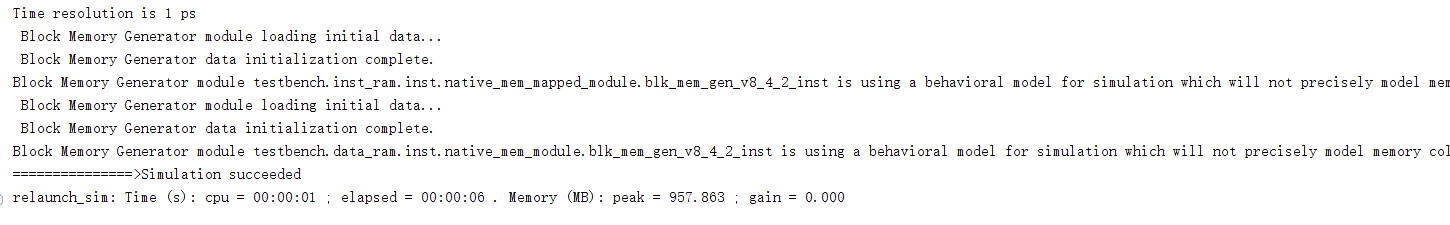
\includegraphics[width=0.8\textwidth]{r3.png}
    \label{图5}
\end{figure}
\begin{figure}[htbp]
    \centering
    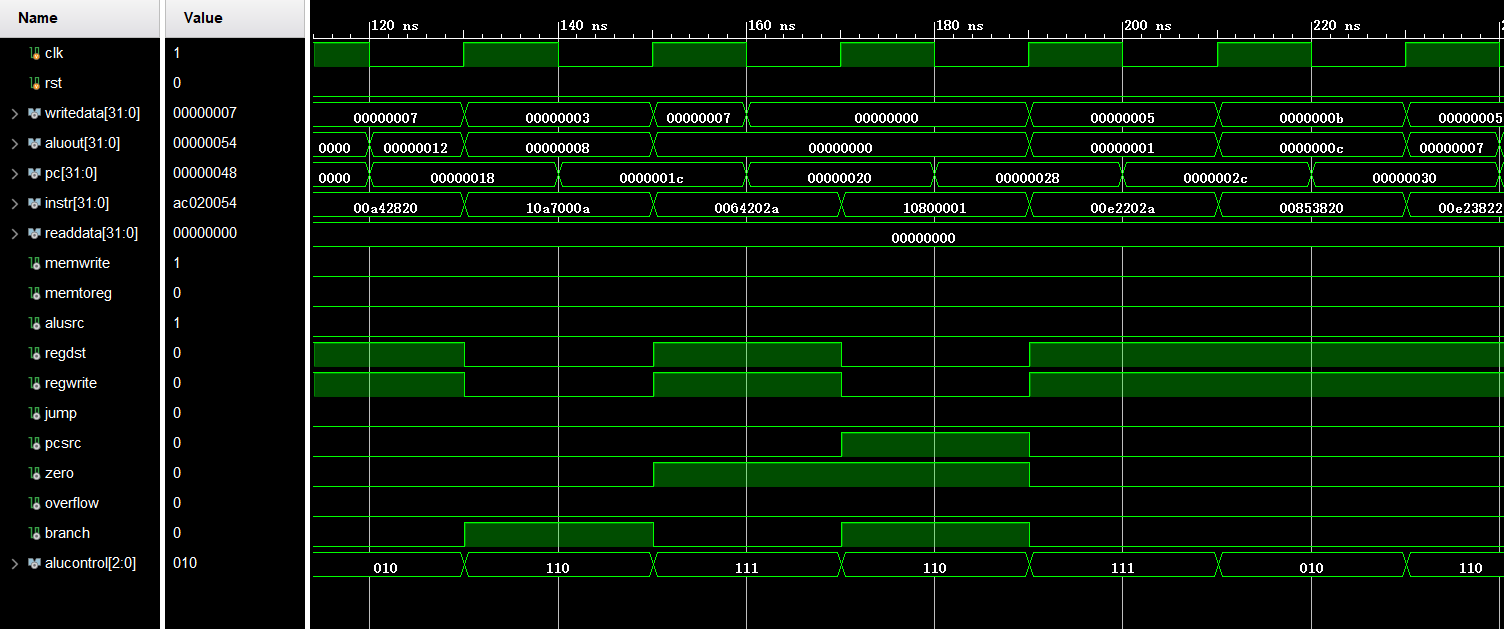
\includegraphics[width=0.8\textwidth]{r4.png}
    \label{图6}
\end{figure}
\begin{figure}[htbp]
    \centering
    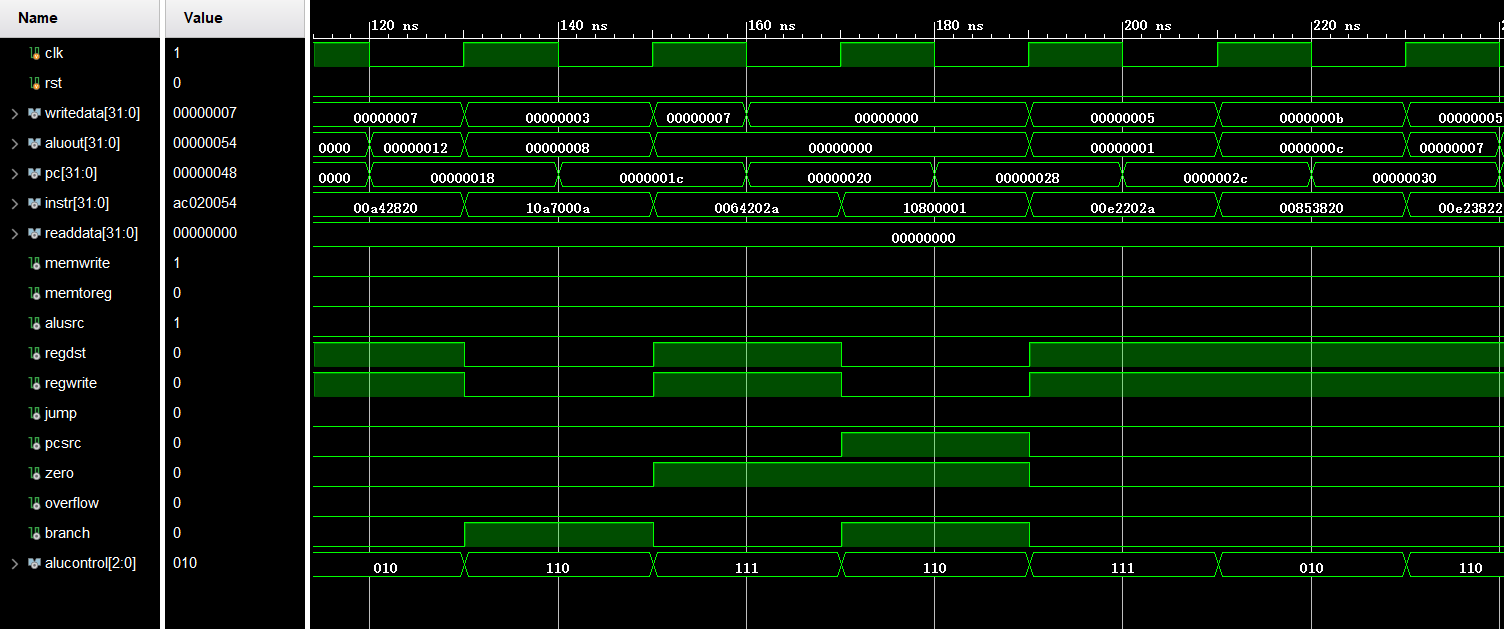
\includegraphics[width=0.8\textwidth]{r4.png}
    \label{图7}
\end{figure}


\subsection{控制台输出}
\begin{figure}[htbp]
    \centering
    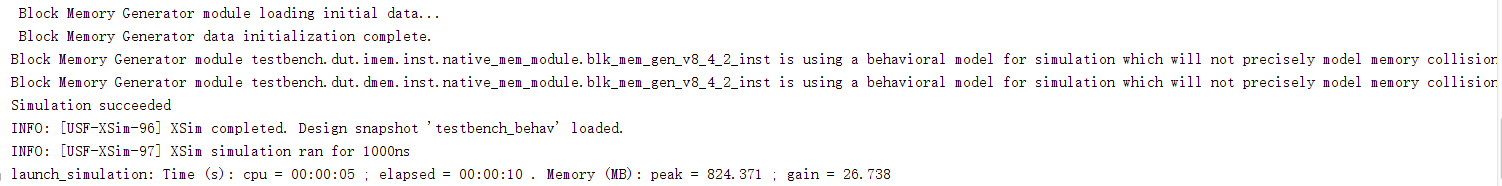
\includegraphics[width=0.8\textwidth]{r2.png}
    \label{图8}
\end{figure}
\newpage
\subsection{结果分析}
\begin{enumerate}
    \item instr = 20020005时为addi指令,将二号寄存器赋初值5,在下降沿regfile有效时,成功写入
    \item instr = 10800001时为beq指令,由于四号寄存器为0,所以branch信号有效,跳转到pc=28位置
    \item instr = ac670044时为sw指令,将七号寄存器保存到80的位置上,aluout为写data\_mem的地址80,写入的值为writedata(RD2) 7
    \item instr = 8c020050时为lw指令,将80位置上的树赋给二号寄存器,aluout为读data\_mem的地址80,readdata的值为7,与上一指令一致,而writedata在下降沿由原来的值5变为7
    \item instr = 08000011时为jump指令,jump信号有效,直接跳转到pc=44的位置
\end{enumerate}